\chapter{随机变量及其分布}

\section{随机变量的分布函数}

\subsection{随机变量}

\begin{definition}
    设随机试验 $E$ 的样本空间为 $\varOmega=\{\omega\}$. 如果对于每一个 $\omega\in\varOmega$,都有一个实数 $X(\omega)$ 与之对应,则称 $X=X(\omega)$ 为\textbf{随机变量}(random variable).
\end{definition}

随机变量常用大写字母 $X,Y,Z$ 等表示.

\subsection{分布函数}

\begin{definition}
    设 $X$ 是一个随机变量,对于任意实数 $x$,令 $F(x)=P\{X \leqslant x\}$,称 $F(x)$ 为随机变量 $X$ 的\textbf{分布函数}(cumulative distribution function).
\end{definition}

随机变量 $X$ 的分布函数 $F(x)$ 是定义在 $(-\infty,+\infty)$ 上的函数,是随机事件 $\{X \leqslant x\}$ 发生的概率.分布函数值 $F(a)$ 表示 $X$ 落在区间 $(-\infty,a]$ 上的概率.

分布函数的基本性质如下.

\setcounter{propertyname}{0}

\begin{property}
    对于任意实数 $x$,有 $0 \leqslant F(x) \leqslant 1$.
\end{property}

\begin{property}
    对于任意实数 $x_1,x_2\, (x_1<x_2)$,有 $P\{x_1 < X \leqslant x_2\}=F(x_2)-F(x_1)$.
\end{property}

\begin{myproof}
    对于任意实数 $x_1,x_2\, (x_1<x_2)$,由于
    $$
    \{x_1 < X \leqslant x_2\} = \{X \leqslant x_2\} - \{X \leqslant x_1\}
    $$
    所以有
    $$
    \begin{aligned}
        P\{x_1 < X \leqslant x_2\} &= P\{X \leqslant x_2\} - P\{X \leqslant x_1\}\\
        &= F(x_2)-F(x_1)
    \end{aligned}
    $$
\end{myproof}

\begin{property}
    \begin{gather*}
        F(-\infty)= \lim_{x \to -\infty} F(x)=0\\
        F(+\infty)= \lim_{x \to +\infty} F(x)=1
    \end{gather*}
\end{property}

\begin{property}
    $F(x)$ 处处右连续,即 $F(x^+)=F(x)$.
\end{property}

\begin{property}
    $F(x)$ 是一个单调不减函数.
\end{property}

\begin{myproof}
    对于任意实数 $x_1,x_2\, (x_1<x_2)$,有
    $$
    F(x_2)-F(x_1) = P\{x_1 < X \leqslant x_2\} \geqslant 0
    $$
    因此 $F(x)$ 是单调不减函数.
\end{myproof}

\section{离散型随机变量及其概率分布}

\begin{definition}
    如果一个随机变量 $X$ 所有可能取到的不相同的值是有限个或可列无限多个,并且以确定的概率取这些不同的值,则称 $X$ 为\textbf{离散型随机变量}(discrete random variable).
\end{definition}

\begin{definition}
    设离散型随机变量 $X$ 所有可能取的值为 $x_k\, (k=1,2,\cdots)$,$X$ 取各个可能值的概率,即事件 $\{X=x_k\}$ 的概率为
    \begin{equation} \label{equation:distribution}
        P\{X=x_k\} = p_k \quad k=1,2,\cdots
    \end{equation}
    并且 $p_k$ 满足以下两个条件:
    \begin{enumerate}
        \item $p_k \geqslant 0$;
        \item $\displaystyle\sum_{k=1}^\infty p_k=1$,
    \end{enumerate}
    则称式 \eqref{equation:distribution} 为离散型随机变量 $X$ 的\textbf{概率分布}(probability distribution)或\textbf{分布律}.
\end{definition}

概率分布也可以用如下的表格来表示:
\begin{table*}[htbp]
    \centering

    \begin{tabular}{c | c c c c c}
        \hline
        $X$ & $x_1$ & $x_2$ & $\cdots$ & $x_k$ & $\cdots$ \\
        \hline
        $P$ & $p_1$ & $p_2$ & $\cdots$ & $p_k$ & $\cdots$ \\
        \hline
    \end{tabular}
\end{table*}

概率分布反映了离散型随机变量的统计规律性.

对于任意实数 $x$,随机事件 $\{X \leqslant x\}$ 可以表示成 $\displaystyle\bigcup_{x_k \leqslant x} \{X=x_k\}$. 由于 $x_k\, (k=1,2,\cdots)$ 互不相同,根据概率的可加性,可得离散型随机变量 $X$ 的分布函数为
$$
F(x) = P\{X \leqslant x\} = \sum_{x_k \leqslant x} P\{X=x_k\} = \sum_{x_k \leqslant x} p_k
$$

\section{连续型随机变量及其概率密度}

\begin{definition} \label{def:f(x)}
    对于随机变量 $X$ 的分布函数 $F(x)$,如果存在非负函数 $f(x)$,使得对任意的 $x$,都有 $F(x)=\displaystyle\int_{-\infty}^x f(t)\,\text{d}t$,则称随机变量 $X$ 是\textbf{连续型随机变量}(continuous random variable),其中函数 $f(x)$ 叫做 $X$ 的\textbf{概率密度函数}(probability density function),简称为\textbf{概率密度}(probability density),记作 $X \sim f(x)$.
\end{definition}

由定义 \ref{def:f(x)} 可知,连续型随机变量的分布函数处处连续.

概率密度 $f(x)$ 的性质如下.

\setcounter{propertyname}{0}

\begin{property} \label{prop:f(x)>=0}
    $f(x) \geqslant 0$
\end{property}

\begin{property} \label{prop:f(x):integral=1}
    $\displaystyle\int_{-\infty}^{+\infty} f(x)\,\text{d}x = 1$
\end{property}

满足性质 \ref*{prop:f(x)>=0} 与性质 \ref*{prop:f(x):integral=1} 的函数 $f(x)$ 必然是某随机变量的概率密度.

\begin{property}
    对于任意实数 $a,b\,(a<b)$,有
    $$
    P\{a < X \leqslant b\}=F(b)-F(a)=\int_a^b f(x)\,\text{d}x
    $$
\end{property}

由以上性质可知,概率密度曲线总是位于 $x$ 轴上方,并且介于它和 $x$ 轴之间的面积等于 1;随机变量落在区间 $(a,b]$ 的概率 $P\{a < X \leqslant b\}$ 等于区间 $(a,b]$ 上曲线 $y=f(x)$ 之下的曲边梯形的面积.

\begin{property} \label{prop:F'(x)=f(x)}
    如果 $f(x)$ 在点 $x$ 处连续,则有 $F'(x)=f(x)$.
\end{property}

由性质 \ref*{prop:F'(x)=f(x)} 可知,在 $f(x)$ 的连续点有
$$
\begin{aligned}
    f(x) &= \lim_{\Delta x \to 0^+} \dfrac{F(x + \Delta x)-F(x)}{\Delta x}\\
    &= \lim_{\Delta x \to 0^+} \dfrac{P\{x < X \leqslant x + \Delta x\}}{\Delta x}
\end{aligned}
$$
可见概率密度反映了随机变量在点 $x$ 处概率分布的密集程度.$f(x)$ 的大小能反映出随机变量 $X$ 在点 $x$ 附近取值的可能性大小,即概率的大小.因此,用概率密度描述连续型随机变量的分布比用分布函数更直观.当不考虑高阶无穷小时,有
$$
P\{x < X \leqslant x + \Delta x\} \approx f(x) \Delta x
$$

对于 $X$ 的任意一个可取的值 $x$,设 $\Delta x > 0$,由于事件 $\{X=x\} \subseteq \{x - \Delta x < X \leqslant x\}$,因此有
$$
0 \leqslant P\{X=x\} \leqslant P\{x - \Delta x < X \leqslant x\} = F(x)-F(x-\Delta x)
$$
令 $\Delta x \to 0$,可得
$$
P\{X=x\}=0
$$
因此,连续型随机变量取任意指定实数的概率均为零.据此,在计算连续型随机变量在某一区间取值的概率时,可以不区分该区间是开区间或闭区间或半开半闭区间,即有
$$
P\{x_1 < X < x_2\} = P\{x_1 \leqslant X \leqslant x_2\} = \int_{x_1}^{x_2} f(x)\,\text{d}x
$$

由上述结论可知,概率为 0 的事件未必是不可能事件.

\section{常用的分布}

\subsection{(0-1)分布}

\begin{definition}
    如果离散型随机变量 $X$ 只取 0 与 1 两个值,其概率分布为
    $$
    P\{X=0\}=1-p, \; P\{X=1\}=p, \; 0<p<1
    $$
    或写成
    $$
    P\{X=k\}=p^k (1-p)^{1-k}, \; k=0,1, \; 0<p<1
    $$
    则称随机变量 $X$ 服从参数为 $p$ 的\textbf{(0-1)分布}或\textbf{两点分布}(two-point distribution).
\end{definition}

服从两点分布的随机变量 $X$ 的概率分布也可以写成
\begin{table*}[htbp]
    \centering

    \begin{tabular}{c | c c}
        \hline
        $X$ & 0 & 1 \\
        \hline
        $P$ & $1-p$ & $p$ \\
        \hline
    \end{tabular}
\end{table*}

\subsection{二项分布}

在 $n$ 重伯努利试验中,如果以 $X$ 表示事件 $A$ 出现的次数,则 $X$ 是一个离散型随机变量,它的所有可能取值是 $0,1,2,\cdots,n$.设 $P(A)=p\,(0<p<1)$,则由二项概率公式(式 \eqref{equation:binomial})可得
$$
P\{X=k\}=C_n^k p^k (1-p)^{n-k}, \; k=0,1,\cdots,n
$$

\begin{definition} \label{def:binomial distribution}
    如果随机变量 $X$ 的概率分布为
    $$
    P\{X=k\}=C_n^k p^k (1-p)^{n-k}, \; k=0,1,\cdots,n
    $$
    则称随机变量 $X$ 服从参数为 $n,p$ 的\textbf{二项分布}(binomial distribution),记作 $X \sim B(n,p)$.
\end{definition}

由定义 \ref{def:binomial distribution} 可得
\begin{gather*}
    P\{X=k\} \geqslant 0\\
    \sum_{k=0}^n P\{X=k\} = \sum_{k=0}^n C_n^k p^k (1-p)^{n-k} = [p+(1-p)]^n=1
\end{gather*}

特别地,当 $n=1$ 时,二项分布 $B(1,p)$ 的概率分布为
$$
P\{X=k\} = p^k (1-p)^{1-k}, \; k=0,1
$$
这就是(0-1)分布. 因此,(0-1)分布是二项分布的特例.

\subsection{泊松分布}

\begin{definition}
    如果离散型随机变量 $X$ 的所有可能取值为 $0,1,2,\cdots$,并且
    $$
    P\{X=k\} = \dfrac{\lambda^k e^{-\lambda}}{k!}, \; k=0,1,2\cdots
    $$
    其中 $\lambda > 0$ 是常数,则称随机变量 $X$ 服从参数为 $\lambda$ 的\textbf{泊松分布}(poisson distribution),记作 $X \sim P(\lambda)$ 或 $X \sim \pi(\lambda)$.
\end{definition}

易知
\begin{gather*}
    \dfrac{\lambda^k e^{-\lambda}}{k!} > 0\\
    \sum_{k=0}^\infty \dfrac{\lambda^k e^{-\lambda}}{k!} = e^{-\lambda} \sum_{k=0}^\infty \dfrac{\lambda^k}{k!} = e^{-\lambda} e^{\lambda}=1
\end{gather*}

\begin{figure}[htbp]
    \centering

    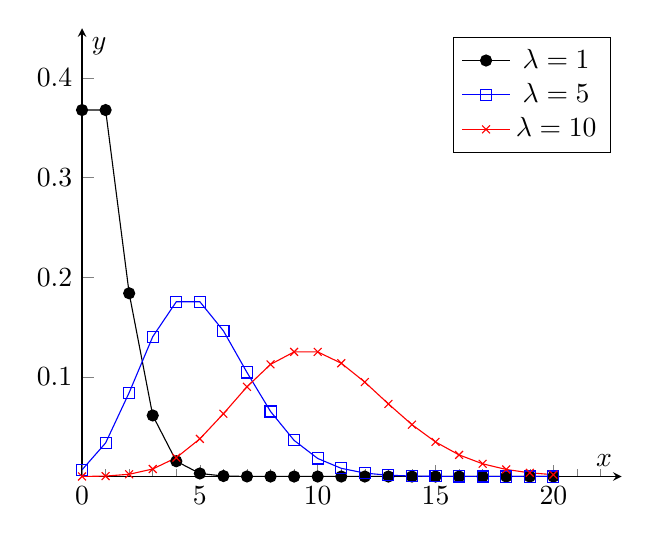
\begin{tikzpicture}
        \begin{axis}[xlabel=$x$, ylabel=$y$,
            axis lines=center,
            tick align=inside,
            xtick distance=5, ytick distance=0.1,
            minor x tick num=4,
            extra x ticks={0},
            xmin=0, xmax=22.9,
            ymin=0, ymax=0.45]
            \addplot[domain=0:20, samples=21, mark=*]{exp(-1)/(x!)};
            \addplot[domain=0:20, samples=21, mark=square, color=blue]{5^x * exp(-5) / (x!)};
            \addplot[domain=0:20, samples=21, mark=x, color=red]{10^x * exp(-10) / (x!)};

            \legend{$\lambda=1$, $\lambda=5$, $\lambda=10$}
        \end{axis}
    \end{tikzpicture}

    \caption{泊松分布}
\end{figure}

\begin{theorem}[(泊松定理)]
    设 $\lambda > 0$ 是常数,$n$ 为任意正整数,$n p_n=\lambda$,则对任一固定的非负整数 $k$,有
    $$
    \lim_{n\to\infty} C_n^k p_n^k (1-p_n)^{n-k} = \dfrac{\lambda^k e^{-\lambda}}{k!}
    $$
\end{theorem}

\begin{myproof}
    因为 $n p_n=\lambda$,故 $p_n=\dfrac{\lambda}{n}$,从而对于任意固定的非负整数 $k$,有
    $$
    \begin{aligned}
        & C_n^k p_n^k (1-p_n)^{n-k}\\
        =\ & \dfrac{n(n-1) \cdots (n-k+1)}{k!} \left( \dfrac{\lambda}{n} \right)^k \left( 1-\dfrac{\lambda}{n} \right)^{n-k}\\
        =\ & \dfrac{\lambda^k}{k!} \left[ 1 \times \left( 1-\dfrac{1}{n} \right) \left( 1-\dfrac{2}{n} \right) \cdots \left( 1-\dfrac{k-1}{n} \right) \right] \left( 1-\dfrac{\lambda}{n} \right)^n \left( 1-\dfrac{\lambda}{n} \right)^{-k}
    \end{aligned}
    $$

    对于固定的 $k$,当 $n\to\infty$ 时,有
    \begin{gather*}
        1 \times \left( 1-\dfrac{1}{n} \right) \left( 1-\dfrac{2}{n} \right) \cdots \left( 1-\dfrac{k-1}{n} \right) \to 1 \\
        \left( 1-\dfrac{\lambda}{n} \right)^n \to e^{-\lambda} \\
        \left( 1-\dfrac{\lambda}{n} \right)^{-k}\to 1
    \end{gather*}
    所以
    $$
    \lim_{n\to\infty} C_n^k p_n^k (1-p_n)^{n-k} = \dfrac{\lambda^k e^{-\lambda}}{k!}
    $$
\end{myproof}

由于 $n p_n=\lambda$,意味着当 $n$ 很大时 $p_n$ 必定很小.因此,泊松定理表明,当 $n$ 很大而 $p$ 很小时,有下面的近似公式
$$
C_n^k p^k (1-p)^{n-k}\approx \dfrac{\lambda^k e^{-\lambda}}{k!}
$$
其中 $\lambda=np$.也就是说,对于二项分布 $B(n,p)$,当 $n$ 很大而 $p$ 很小时,近似为泊松分布 $P(np)$.